\expandafter\newcommand\csname dataBernoulliNBmetrictab\endcsname{
\begin{table}[H]
\begin{tabular}
{| 
 p{\dimexpr0.2\textwidth-2\tabcolsep-\arrayrulewidth\relax}| 
 p{\dimexpr0.2\textwidth-2\tabcolsep-\arrayrulewidth\relax}| 
 p{\dimexpr0.2\textwidth-2\tabcolsep-\arrayrulewidth\relax}| 
 p{\dimexpr0.2\textwidth-2\tabcolsep-\arrayrulewidth\relax}| 
 p{\dimexpr0.2\textwidth-2\tabcolsep-\arrayrulewidth\relax}| 
}\hline 
\textbf{} &\textbf{f1-score} &\textbf{precision} &\textbf{recall} &\textbf{support} \\ \hline 
CANDIDATE &0.279 &0.321 &0.247 &170.0 \\ \hline 
CONFIRMED &0.564 &0.441 &0.784 &241.0 \\ \hline 
FALSE POSITIVE &0.676 &0.884 &0.547 &391.0 \\ \hline 
accuracy &0.555 &0.555 &0.555 &0.555 \\ \hline 
macro avg &0.506 &0.548 &0.526 &802.0 \\ \hline 
weighted avg &0.558 &0.631 &0.555 &802.0 \\ \hline 
\end{tabular} 
\end{table}
}
\begin{figure}[H]
                \centering
                \begin{subfigure}{.49\textwidth}
                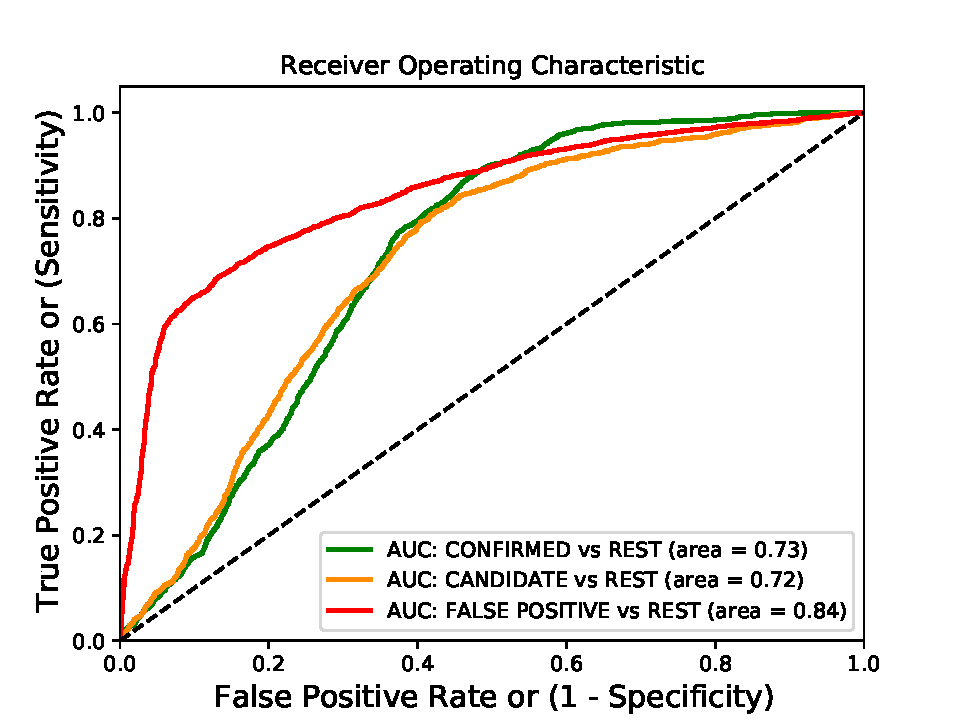
\includegraphics[width = 1\textwidth]{data/BernoulliNB_overfit_roc.pdf}
                \end{subfigure}
                \begin{subfigure}{.49\textwidth}
                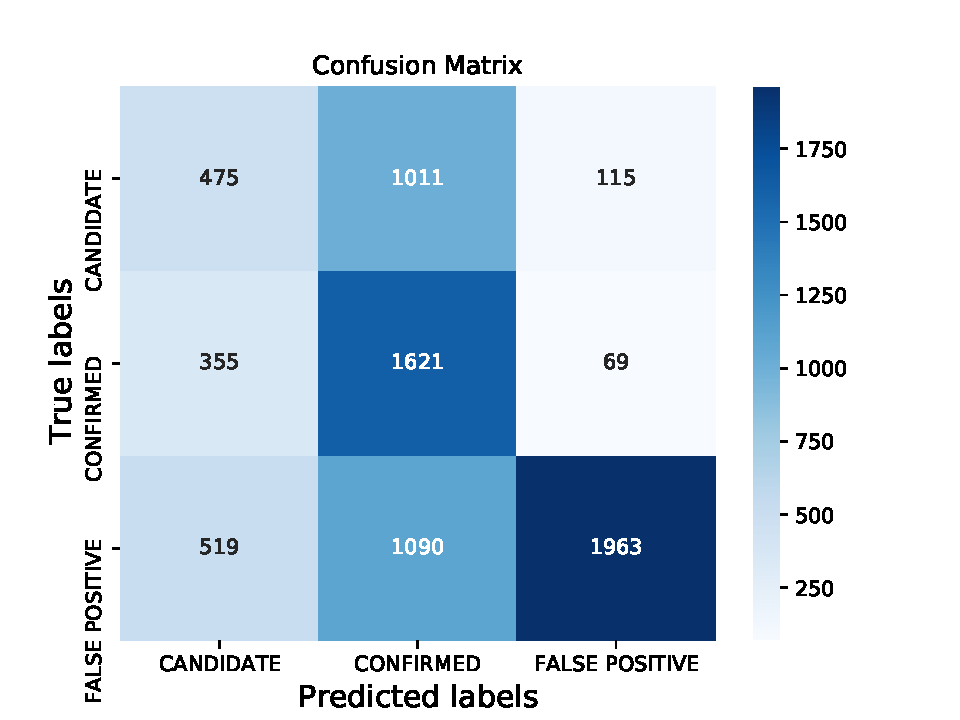
\includegraphics[width = 1\textwidth]{data/BernoulliNB_overfit_cm.pdf}
                \end{subfigure}
                \begin{subfigure}{.49\textwidth}
                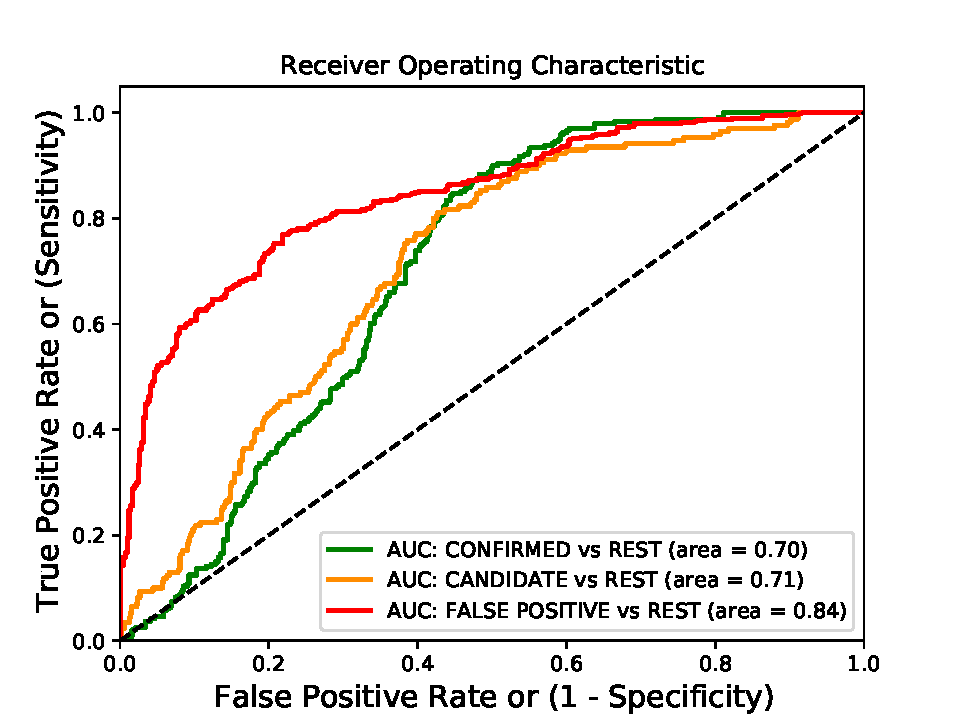
\includegraphics[width = 1\textwidth]{data/BernoulliNB_roc.pdf}
                \end{subfigure}
                \begin{subfigure}{.49\textwidth}
                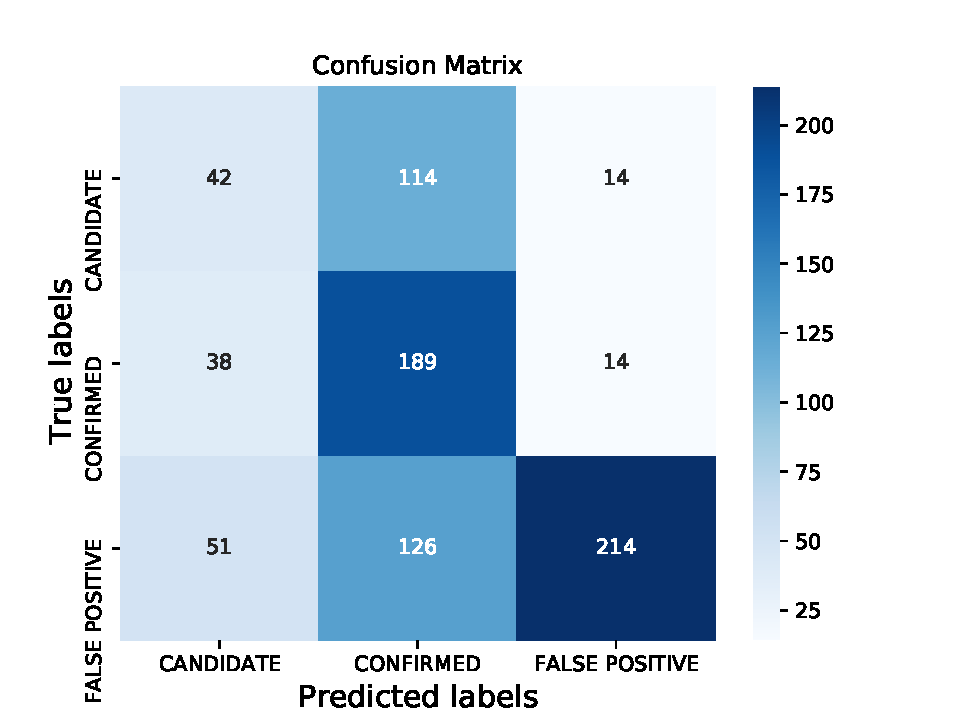
\includegraphics[width = 1\textwidth]{data/BernoulliNB_cm.pdf}
                \end{subfigure}
                \begin{subfigure}{1\textwidth}
                \csname dataBernoulliNBmetrictab\endcsname
                \end{subfigure}
                \caption{BernoulliNB: Top Row: overfit test. Middle and bottom row test data}
                \label{fig:data/BernoulliNB_roc}
                \end{figure}